\documentclass[]{article}
\usepackage{lmodern}
\usepackage{amssymb,amsmath}
\usepackage{ifxetex,ifluatex}
\usepackage{fixltx2e} % provides \textsubscript
\ifnum 0\ifxetex 1\fi\ifluatex 1\fi=0 % if pdftex
  \usepackage[T1]{fontenc}
  \usepackage[utf8]{inputenc}
\else % if luatex or xelatex
  \ifxetex
    \usepackage{mathspec}
    \usepackage{xltxtra,xunicode}
  \else
    \usepackage{fontspec}
  \fi
  \defaultfontfeatures{Mapping=tex-text,Scale=MatchLowercase}
  \newcommand{\euro}{€}
\fi
% use upquote if available, for straight quotes in verbatim environments
\IfFileExists{upquote.sty}{\usepackage{upquote}}{}
% use microtype if available
\IfFileExists{microtype.sty}{%
\usepackage{microtype}
\UseMicrotypeSet[protrusion]{basicmath} % disable protrusion for tt fonts
}{}
\ifxetex
  \usepackage[setpagesize=false, % page size defined by xetex
              unicode=false, % unicode breaks when used with xetex
              xetex]{hyperref}
\else
  \usepackage[unicode=true]{hyperref}
\fi
\usepackage[usenames,dvipsnames]{color}
\hypersetup{breaklinks=true,
            bookmarks=true,
            pdfauthor={Anders Rydbirk},
            pdftitle={Algorithms for Ricochet Robots},
            colorlinks=true,
            citecolor=blue,
            urlcolor=blue,
            linkcolor=magenta,
            pdfborder={0 0 0}}
\urlstyle{same}  % don't use monospace font for urls
\usepackage{longtable,booktabs}
\setlength{\parindent}{0pt}
\setlength{\parskip}{6pt plus 2pt minus 1pt}
\setlength{\emergencystretch}{3em}  % prevent overfull lines
\providecommand{\tightlist}{%
  \setlength{\itemsep}{0pt}\setlength{\parskip}{0pt}}
\setcounter{secnumdepth}{5}

\title{Algorithms for Ricochet Robots}
\author{Anders Rydbirk}
\date{}
\usepackage{fancyhdr}
\pagestyle{fancy}
\usepackage{graphicx,grffile}
\usepackage{lscape}
\usepackage[graphicx]{realboxes}
\makeatletter
\def\maxwidth{\ifdim\Gin@nat@width>\linewidth\linewidth\else\Gin@nat@width\fi}
\def\maxheight{\ifdim\Gin@nat@height>\textheight\textheight\else\Gin@nat@height\fi}
\makeatother
\setkeys{Gin}{width=\maxwidth,height=\maxheight,keepaspectratio}

% Redefines (sub)paragraphs to behave more like sections
\ifx\paragraph\undefined\else
\let\oldparagraph\paragraph
\renewcommand{\paragraph}[1]{\oldparagraph{#1}\mbox{}}
\fi
\ifx\subparagraph\undefined\else
\let\oldsubparagraph\subparagraph
\renewcommand{\subparagraph}[1]{\oldsubparagraph{#1}\mbox{}}
\fi

\begin{document}
\maketitle
\begin{abstract}
This is a pandoc test . . .

another line of abstract!
\end{abstract}

{
\hypersetup{linkcolor=black}
\setcounter{tocdepth}{3}
\tableofcontents
}
\newpage

\section{Introduction}\label{introduction}

Optimizing a single entity's cost is the most common approach in path
finding problems. However, the board game \emph{Ricochet Robots}
presents a rather unusual case where multiple entities coorperate for a
single entity to reach the goal at minimal cost. Usually, the map is
considered static in path finding problems, however, in \emph{Ricochet
Robots} the map is altered for each move of an entity, resulting in a
new problem. With multiple possible moves for each map, the search space
increases rapidly.

The goal of this project is to survey and design state-of-the-art
algorithms within graph search and dynamic programming. I will survey
existing solutions for \emph{Ricochet Robots} and, based on the
experience, design and implement new state-of-the-art algorithms. I will
be implementing prototypes of each algorithm and analyse and evaluate
each algorithm from both a theoretical and practival perspective.

\subsection{Ricochet Robots}\label{ricochet-robots}

Ricochet Robots is played on a board consisting of \(16 \cdot 16\) tiles
with obstacles scattered on the board as seen in figure
\ref{fig:example}. The board contains 17 goals. Four robots in different
colors are randomly placed on the board at the beginning of the game.
The robots cannot be positioned on the same field or on a goal field.
Each goal is colored in relation to one of the four robots except for
one of the goals which is reachable by all colors. The game is played by
solving the individual goal sequentially. The objective of the game is
to identify the minimum number of moves on order for the corresponding
robot to land on the given goal. All robot can be moved and all robots
can be used as obstacles for the other robots.

A round starts with picking a goal to reach. All players can declare
they are able to reach the goal in a specific number of moves. When the
first player declares a number, all the other players have one minute to
find a lower (and more efficient) number of moves. If so, the player
calling a lower number of moves demonstrates his/her solution and wins
the round, and if not, the declaring player wins the round. The game
continues until all 17 goals have been played. The game is now over and
the aggregated winner is found.

\begin{figure}[htb]
\centering
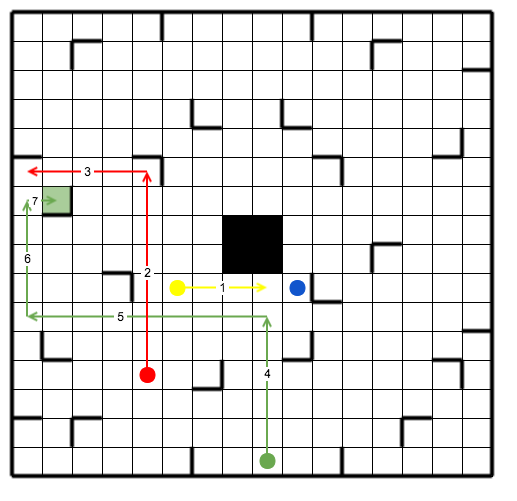
\includegraphics[width=0.6\linewidth]{img/example.png}
\caption{An example of \emph{Ricochet Robots} where the green robot has to reach the goal at (7,2). The minimum number of moves is seven, and multiple solutions exist. The number on each arrow indicates the order of moves. Thus, the yellow robot moves first so that the green robot can bounce off it on the fourth move.}
\label{fig:example}
\end{figure}

Moving the robots is one of the characteristic parts of the game. A
robot moves like a rook in chess, but it moves in a direction until it
hits an obstacle or another robot. This counts as one move. Thus, a
robot cannot stop on any of the intermediate fields. All robots can be
moved and used as obstacles for the other robots. An example is given in
figure \ref{fig:example}. The robots can move in four directions. As a
result, for each move, \(|directions| \cdot |robots| = 16\) new possible
moves can be made. This is also refered to as the branching factor.
However, as the robots move they are adjacent to at least one obstacle,
and the branching factor appromixates 12. The number of possible
combinations for a given game is given by \(12^k\) where \emph{k} is the
required number of moves to reach the goal. Given the exponential growth
in possible combinations, the game presents three major challenges for
both players and computers:

\begin{enumerate}
\def\labelenumi{\arabic{enumi}.}
\tightlist
\item
  Finding a valid solution
\item
  Guaranteeing an optimal solution
\item
  Solving the game in reasonable time
\end{enumerate}

The game has been proven NP-Hard\textbf{\emph{REFERENCE}} which
underlines the complexity of the game is an exponential function of the
required number of moves. Precomputing each and every robot combination
for each board is infeasible given the high number of robot combinations
and the complexity of each game. Thus, tradeoffs between solving the
game optimally and solving the game in reasonable time are the core of
developing algorithms for this game.

\subsection{Baseline}\label{baseline}

The following definitions are general for all algorithms.

Let \emph{b} be the branching factor, and let \emph{k} be the number of
moves to reach the goal. The number of possible moves in each game is
given by \(b^k\).

Let \emph{n} be the dimensions of the board where \emph{n = 16}. Let
\emph{F} be the set of fields where \emph{F{[}i,j{]}} refers to the
field at the \emph{i'th} row and the \emph{j'th} column starting from
the top-left corner. Each field contains information about obstacles in
each direction. Let \emph{R} be the set of robots, let \emph{GR} be the
Goal Robot to reach the goal and let \emph{OR} be the set of Obstacle
Robots \(\in R - \{GR\}\).

A robot state refers to the position of the robot and the required moves
to reach the state, while a game state refers to the complete set of
robot states for a current configuration.

Let \emph{b} be the branching factor describing the number of possible
moves for each game state and let \emph{k} be the minimum number of
moves required for solving a given game.

The set of directional indicators \emph{D} refers to the possible
directions on the gameboard. Thus,
\(D = \{ North, East, South, West \}\).

Each algorithm is given the board of fields \emph{F}, the set of robots
\emph{R} and the goal to reach \emph{G} as input.

\subsection{Previous Solutions}\label{previous-solutions}

A few solutions exist for \emph{Ricochet Robots} and the two most common
are described below.

\subsubsection{Naive Algorithm}\label{naive-algorithm}

The naive algorithm searches the entire search tree in an incremental
order and guarantees an optimal solution. The board representation is a
two dimensional array with an additional attribute for each field
indicating if a robot stands on the given field. A first-in, first-out
queue is used for keeping track of the to-be processed game states.
Since this solution would never be feasable for solutions requiring more
than a couple moves, a hash table is introduced to keep track of already
searched game states. Therefore, duplicate game states will be pruned
from the search tree.

To move a robot, all fields in a given direction is processed until an
obstacle is met. It uses \(O(n)\) time. This is done for each robot for
each direction for each game state. Processing each game state includes
the branching factor and uses \(O(b \cdot n)\) time.

Solving a given configuration uses
\(O(b^k \cdot b \cdot n) = O(b^{k+1} \cdot n)\) time. The algorithm uses
\(O(n^2)\) space for the additional attribute for each field, \(O(b^k)\)
space for the queue and \(O \Big(\sum\limits_{i=1}^k b^i \Big)\)
\emph{\textasciitilde{}} \(O(b^k)\) for the hash table. The worst case
space impact of the algorithm is \(O(b^k + n^2)\).

Each robot is adjacent to at least one obstacle after the initial move.
Therefore the branching factor is given by
\(b = |R| \cdot (|D|-1) = 12\).

\subsubsection{Iterative Deepening Depth First Search
(IDDFS)}\label{iterative-deepening-depth-first-search-iddfs}

The IDDFS algorithm is claimed to be fastest solver and guarantees an
optimal solution. The algorithm uses the same board representation as
the naive algorithm including the additional attribute for flagging
robot locations. In the following, \emph{h} will refer to the height of
the remaining search for the iteration. Thus, \(h = MAX - depth\), where
\emph{MAX} is the incrementing search limit while \emph{depth} is the
distance to the root in the search tree. The IDDFS includes two
additional pruning techniques:

\begin{enumerate}
\def\labelenumi{\arabic{enumi}.}
\tightlist
\item
  A hash table stores a combination of game state \emph{s} and \emph{h}.
  If \emph{s} has been reached before by the same height, it is pruned
  from the search.
\item
  A two-dimensional array stores the minimum number of moves from each
  field to goal. In the latter, \emph{min{[}i,j{]}} refers to the
  minimum number of moves to goal from position \emph{(i,j)}. It is
  assumed that the robots can change direction without bouncing off an
  obstacle as seen in figure \ref{fig:minmoves}. If \(min[GR] > h\) the
  search is pruned. If \(h = min[GR]\) only the \emph{GR} is processed
  further in the search tree.
\end{enumerate}

\begin{figure}[htb]
\centering
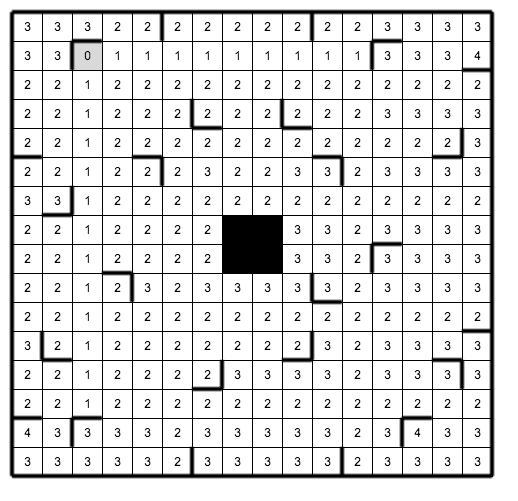
\includegraphics[width=0.6\linewidth]{img/min_moves.png}
\caption{The minimum number of moves for each field to reach the goal at (2,3) colored in grey. All moves assumes optimal placement of other robots.}
\label{fig:minmoves}
\end{figure}

The minimum moves for each field is computed with the goal as the root.
The number of moves for the root is set to 0. Each direction is
processed incrementing the number of moves with 1. For each direction,
all fields is processed until an obstacle or a field with a lower
minimum number of moves is met. Due to this incremental movement, every
field is only queued once but can be visited several times during the
computation. When processing a single field, only two directions is
relevant since the field was discovered from one of the other two
directions and therefore these directions are guaranteed to be more
optimal. When processing a single field, only \(O(n)\) fields are
visited. Since all fields are queued exactly once, the minimum moves are
computed in \(O(n^2 \cdot n) = O(n^3)\) time and uses \(O(n^2)\) space.

Finding the optimal solution uses \(O(b^k \cdot n + n^3)\) time.
However, the space impact of the search itself is only \(O(k)\) since
the algorithm is recursive. The space analysis of the hash table is the
same as in the naive algorithm. The worst case space impact is
\(O(b^k+k+n^2) = O(b^k+n^2)\).

\section{Solutions}\label{solutions}

In the following, I will describe my solutions to the problem presented
by \emph{Ricochet Robots} and analyse each for running time and space
impact.

\subsection{Stateless}\label{stateless}

The stateless algorithm is an attempt to solve the game without keeping
track of each game state. The obvious advantage of this is to eliminate
impact of the branching factor on the running time. The algorithm does
not guarantee an optimal solution. Instead, it stores information about
every time a robot interacts with a field. The interaction can be split
in two - when the robot moves over the field, or when it lands on the
field. In the latter example, landing on a field is denoted as a
\emph{final state} while moving over a field is denoted as an
\emph{intermediate state}. The algorithm assumes that every field can
only have one final state for each robot, and only one intermediate
state for each combination of direction and color.

Final states are queued in a min-heap queue ordered by the number of
moves. These states represent only a single state of a robot, thus for
each element in the queue, only one robot is processed. The robot is
moved in all directions and a new state are created for each visited
field if no redundant state already exist for the given field. The
algorithm terminates when there are no more robot states to process,
whereafter the best result is returned.

\subsubsection{The Stateless Algorithm}\label{the-stateless-algorithm}

Let \emph{S{[}i,j{]}} refer to the element storing states for
\emph{F{[}i,j{]}}. \emph{S{[}i,j{]}} is instantiated at the first visit
to \emph{F{[}i,j{]}}. Each \(s \in S\) stores final states in a hash
table using the color of the robot as key. In addition, \emph{s} stores
all intermediate states in a hash table using the direction of the robot
move as the key. Finally, \emph{s} stores if a robot starts on the
field.

\paragraph{Moving And States}\label{moving-and-states}

Moving a robot determines the state for each field processed. The state
depends upon the next field to process if it is possible to move
further. Four cases are taken into consideration when moving robot
\emph{r}, and all four cases are evaluated for each step until an
obstacle is met. In the following, \emph{a} will refer to the adjacent
field in direction \emph{d}:

\begin{enumerate}
\def\labelenumi{\arabic{enumi}.}
\tightlist
\item
  \emph{F{[}i,j{]}} cannot move in direction \emph{d}. A final state
  \emph{f} is added to \emph{S{[}i,j{]}}. If a final state did not
  already exist, \emph{f} is added to the queue for future processing.
\item
  \emph{F{[}i,j{]}} can move in direction \emph{d}:

  \begin{enumerate}
  \def\labelenumii{\alph{enumii}.}
  \tightlist
  \item
    No final robot states exist on \emph{a}. Thus, an intermediate state
    is added to \emph{S{[}i,j{]}} and \emph{a} is processed next.
  \item
    A final robot state exist on \emph{a} and its color does not match
    the color of robot \emph{r}. The final state \emph{f} is set to
    depend upon the lowest final state in \emph{S{[}a{]}}, the move
    counts are aggregated and \emph{f} is added to \emph{S{[}i,j{]}}. If
    a final state did not already exist, \emph{f} is added to the queue
    while \emph{a} is processed next.
  \item
    A robot starts on \emph{a}. Case \emph{1.b} is applied, with the
    addition that all the further processing of fields in direction
    \emph{d} for the current \emph{r} will be added one to the number of
    required moves from \emph{a} and forward. This refers to the
    required movement of the starting robot on \emph{a}.
  \end{enumerate}
\end{enumerate}

An initial move is illustrated in figure \ref{fig:stateless} displaying
several of the cases.

\begin{figure}[htb]
\centering
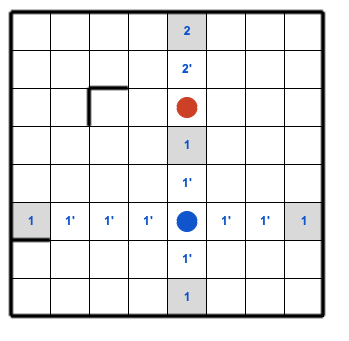
\includegraphics[width=0.6\linewidth]{img/stateless.png}
\caption{The initial move for the blue robot. All grey fields are final states while all fields denoted with an appostrophe are intermediate states. The field of the red robot is also an intermediate state with a value of 2.}
\label{fig:stateless}
\end{figure}

Whenever a new final state \emph{f} is added to the queue, adjacent
fields are searched for intermediate states on collision with \emph{f}.
Let \emph{a} be the adjacent field in direction \emph{d} and let
\emph{d'} be the opposite direction of \emph{d}. All intermediate states
\(i \in I\) where \(i.color \neq f.color \land i.direction = d'\) are
removed from \(S[a]\) and converted to final states that depend upon
\emph{f}. If no final state already exists for the given color in
\(S[a]\), the new final states are added to the queue.

\subsubsection{Analysis}\label{analysis}

The algorithm uses a min-heap queue and insertion and removal uses
\(O(log(m))\) time where \emph{m} refers to the number of elements in
the queue. Since each field is only processed once for every robot,
\(m=O(n^2 \cdot |R|)\). Thus, insertion and removal in the queue uses
\(O(log(|R| \cdot n^2))\) time. Moving a robot uses \(O(2n)\) time like
the naive algorithm. Inserting, lookup, and removal from the hash tables
in \emph{S} uses \(O(1)\) time. Processing each robot state uses
\(O(2n \cdot 2log(|R| \cdot n^2))\) time and the total worst case uses
\(O(n^2 \cdot 2n \cdot 2log(|R| \cdot n^2)) = O(n^3 \cdot log(n^2))\)
time.

In the worst case, each \(s \in S\) stores \(O(|R|)\) final states and
\(O(|D| \cdot |R|)\) intermediate states. The queue contains
\(O(|R| \cdot n^2)\) elements. Therefore, the worst case space impact is
\(O(n^2 \cdot(1 + |R| + |R| \cdot |D|)) = O(n^2)\).

\subsection{Graph v1}\label{graph-v1}

In the following the graph based algorithm will be presented. The
algorithm assumes that all moves by the \emph{OR} can be applied before
the \emph{GR} moves towards the goal. The \emph{GR} can depend on
\emph{OR} states but \emph{OR} can only depend on the starting state of
\emph{GR}. An example of the implications of this assumption is shown in
figure \ref{fig:graph_cases}.

\begin{figure}[htb]
\centering
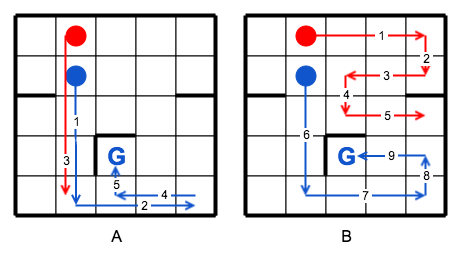
\includegraphics[width=0.6\linewidth]{img/graph_cases.png}
\caption{Case A displays the optimal solution for the given game board while case B is the optimal solution given by the graph algorithm hence case A requires the red robot to move after the initial move of the blue robot.}
\label{fig:graph_cases}
\end{figure}

The algorithm will update the graph with \emph{OR} states and perform a
BFS with the \emph{GR} as the source vertex and stores the result. Like
the naive algorithm, each \emph{OR} are now moved to new positions and
new game states are queued in a first-in, first-out queue. As each level
in the search tree is discovered in an incremental order, the algorithm
guaranties an optimal solution under the given assumption above. As with
the naive algorithm, a hash table is used to prune the search tree.

\subsubsection{The Graph v1 Algorithm}\label{the-graph-v1-algorithm}

Let \emph{G} be the graph representing the board where \emph{G.V} is the
set of vertices in the graph where \emph{G.V{[}i,j{]}} refers to the
vertex at the same position as the corresponding field in
\emph{F{[}i,j{]}}. Let \emph{G.E} be all directional edges in \emph{G}
and let \emph{G.Adj{[}v{]}} refer to all edges where the source is the
vertex \emph{v}. \emph{G} will be represented in a two-dimensional array
with directional edges stored in an adjacency list for each vertex.
Constructing the graph is done in two passes with dynamic programming.
Let \(v \in G.V\) and let \emph{E} = \emph{G.Adj{[}v{]}}. Each edge
\(e \in E\) has a pointer to the next vertex, later referred to as the
child of \emph{e}. Each \emph{e} is also denoted a directional indicator
\(d \in D\). While \emph{v} has at most one edge for each direction,
then \(|E| \leq |D|\) is given.

\paragraph{Construct Graph}\label{construct-graph}

The graph is constructed in two passes, where the first pass is
conducted in a top-down left-to-right approach. The first pass processes
edges in the directions \(d \in \{West, North\}\). Each
\emph{G.V{[}i,j{]}} is added an edge in direction \emph{d} if
\emph{F{[}i,j{]}} has no obstacle in direction \emph{d}. In the case of
\(d \in \{West, North \}\), the respective vertices
\emph{G.V{[}i,j-1{]}} and \emph{G.V{[}i-1,j{]}} will be investigated. As
an example, in case \emph{F{[}i,j{]}} can move in direction \emph{d =
North} and \emph{G.V{[}i-1,j{]}} has an edge in direction \emph{d}, the
child of that edge will also be the child of the edge in direction
\emph{d} for vertex \emph{G.V{[}i,j{]}}. If \emph{G.V{[}i-1,j{]}} has no
edge in direction \emph{d}, \emph{G.V{[}i-1,j{]}} will be the child of
the edge at direction \emph{d} for vertex \emph{G.V{[}i,j{]}}. The
second pass processes edges where \(d \in\) \emph{\{ East, South \}} in
a bottom-up right-to-left approach.

\paragraph{Adapting The Graph}\label{adapting-the-graph}

The graph has to be adapted to the current \emph{OR}'s positions before
the BFS can be applied for the \emph{GR}. Let \emph{(i,j)} be the
position where a robot has to be placed. Let \emph{d} be a direction
from \emph{(i,j)} and let \emph{V} be the set of vertices in direction
\emph{d} which need to be adjusted to the new board configuration. All
vertices in \emph{V} need to update the edges in the opposite direction
of \emph{d}, in the following referred to as \emph{d'}.

Let \emph{v'} be the vertex immidiately adjacent to \emph{G.V{[}i,j{]}}
in direction \emph{d}. Let \emph{E} be the set of
\(e \in G.Adj[V-\{v'\}]\) where \(e.d = d'\). The child property of all
edges in \emph{E} has to be set to \emph{v'} while the edge of \emph{v'}
in direction \emph{d'} has to be removed.

To find the set \emph{V}, the most distant vertex is found and then all
vertices in direction \emph{d'} is processed until \emph{G.V{[}i,j{]}}
is met. Several cases exist when finding the distant vertex which is
illustrated in figure \ref{fig:graph_states} and listed below.

\begin{enumerate}
\def\labelenumi{\arabic{enumi}.}
\tightlist
\item
  \emph{F{[}i,j{]}} cannot move in direction \emph{d}. No edges has to
  be updated.
\item
  \emph{F{[}i,j{]}} can move in direction \emph{d}:

  \begin{enumerate}
  \def\labelenumii{\alph{enumii}.}
  \tightlist
  \item
    \emph{G.V{[}i,j{]}} has no edge in direction \emph{d}. Thus, another
    robot stands on the adjacent field in direction \emph{d}.
  \item
    \emph{G.V{[}i,j{]}} has an edge \emph{e} in direction \emph{d}. The
    field for \emph{e.child} cannot move in direction \emph{d}. Thus,
    \emph{e.child} is the most distant vertex from \emph{G.V{[}i,j{]}}
    in direction \emph{d}.
  \item
    \emph{G.V{[}i,j{]}} has an edge \emph{e} in direction \emph{d}. The
    field for \emph{e.child}, \emph{f}, can move in direction \emph{d}.
    Thus, a robot is present on the adjacent field to \emph{f} in
    direction \emph{d}.
  \end{enumerate}
\end{enumerate}

\begin{figure}[htb]
\centering
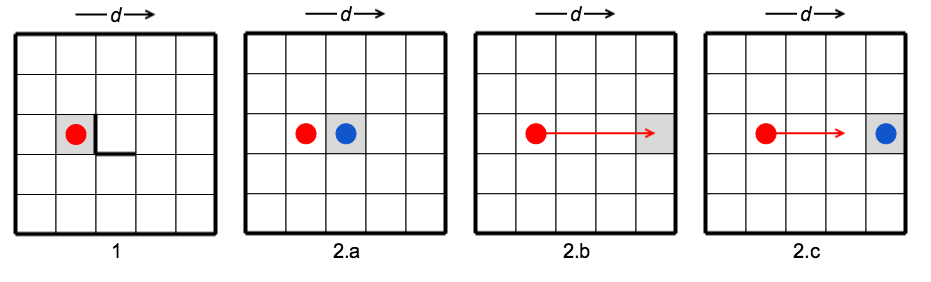
\includegraphics[width=1\linewidth]{img/graph_states.png}
\caption{Each case when updating the graph in direction d. The grey field is the most distant vertex in each case.}
\label{fig:graph_states}
\end{figure}

Given the position \emph{(i,j)}, the fields \emph{F} and the graph
\emph{G}, all directions are processed and the graph is updated with the
new robot position.

Placing and removing a robot from the board involves many of the same
features:

\begin{enumerate}
\def\labelenumi{\arabic{enumi}.}
\tightlist
\item
  Identify relevant directions to investigate.
\item
  Identify relevant vertices to update.
\item
  Add or update edges for all affected vertices.
\end{enumerate}

This functionality will not be described further in this section.

\paragraph{Solver}\label{solver}

In the graph-based solver the search tree is expanded one level at a
time. A first-in, first-out queue is used to store awaiting game states.
In this case, a game state refers to a list of \emph{OR} states and a
property indicating the total number of moves for the given game state.
Like the naive algorithm, a hash table is introduced to track already
processed game states and prunes redundant states.

The solver keeps track of the best known solution so far in \emph{B}.
\emph{B.s} is the game state, \emph{B.bfs} is the result of the BFS and
\emph{B.best} is the combined number of moves for the given solution. A
heuristic function is introduced as the termination state:

\begin{quote}
B is the optimal solution if \(B.best < (s.moves + 2)\), where \emph{s}
is the curent investigated game state. Since the number of moves is
investigated in an incremental order, and since \emph{s} requires at
least one additional move for the goal robot to reach the goal, \emph{s}
will never be a better solution than \emph{B}, and therefore the solver
terminates when this condition is fulfilled.
\end{quote}

The solver instantiates the hash table and constructs the graph. Then
the initial game state is queued and a loop is performed until a
solution is found. For each game state, the heuristic is applied. If the
termination state is not fulfilled, the graph is updated with the the
positions of the \emph{OR} for the given game state. The BFS is applied
and the result of the goal field is found. If it was reached by the
\emph{GR}, the combined result is compared to \emph{B} and updated if
better. Then, the graph is adapted to the position of the \emph{GR}, and
all the \emph{OR} are moved in all directions. The new game states are
validated against the hash table and added to the queue if they are not
redundant. Finally, the robots are all removed from the graph and the
next game state is processed.

\subsubsection{Analysis}\label{analysis-1}

Processing a single field in the construction of the graph uses \(O(1)\)
time, and each pass uses \(O(n^2)\) time. The space impact is given by
\(O(n^2 \cdot |D|) = O(n^2)\) since there is at most one edge per
direction per vertex.

Placing and removing a robot in the graph affects at most \(2 \cdot n\)
vertices. This is the case where the robot is placed where no obstacles
or other robots exist for the given row and column. Finding the distant
vertex uses \emph{O(1)} time. The total time for placing or removing a
robot from the graph uses \(O(2n) = O(n)\) time.

For the solver, each game state processed requires four robot placements
and removals thus \(O(8 \cdot n)\) time. The BFS worst case is given by
the number of vertices and edges, resulting in \(O(n^2 \cdot |D|)\). The
BFS requires a two-dimensional array to keep track of the search
progress using \(O(n^2)\) space. However, this is discarded when the BFS
is completed and the result is returned.

Validating, inserting, and enqueuing a new game state uses \(O(1)\)
time. Moving all robot uses \(O(b)\) time. Therefore, the time used for
each processed game state is
\(O(8 \cdot n + n^2 \cdot |D| + b) = O(n^2)\). In total, the worst case
time usage for the algorithm is \(O(b^k \cdot n^2)\).

The space impact of the queue and the hashtable is \(O(b^k)\). The worst
case space impact of the algorithm is
\(O(n^2 \cdot |D| + 2b^k + n^2) = O(b^k + n^2 \cdot (1 + |D|)) = O(b^k + n^2)\).

After the initial move, each \emph{OR} is adjacent to at least one
obstacle. The branching factor is given by \(b = |OR| \cdot 3 = 9\).

\subsection{Graph v2}\label{graph-v2}

The second version of the graph solver has a few improvements inspired
by the other solvers. In the following, only the additions will be
described.

\subsubsection{Improvements}\label{improvements}

The graph construction, inserting, and removal of robots in the graph is
the same as bescribed for version 1 while the same basic assumptions as
stated in version 1 applies. The additions is focused on the heuristic
function and the BFS while the solver itself has no further additions.

\paragraph{Heuristic Function}\label{heuristic-function}

The heuristic function has been improved to facilitate an earlier
termination of the solver. Using the minimum moves precomputation given
in the IDDFS solver, the heuristic function has been updated to the
following:

\begin{quote}
B is the optimal solution if \(B.best < (s.moves + min[GR])\), where
\emph{s} is the curent investigated game state and \emph{min{[}GR{]}} is
the minimum number of moves from the \emph{GR} to the goal. Given the
incremental order of the search, no possible other solution can reach
goal in fewer moves than the given best, and the condition is satisfied.
\end{quote}

\paragraph{Early Termination of BFS}\label{early-termination-of-bfs}

When a given solution is found, the BFS is still applied until the
heuristic function is satisfied. However, when a solution is found an
upper limit for the possible number of moves is set drastically reducing
the search tree. The following optimizations are an attempt to do so:

\begin{enumerate}
\def\labelenumi{\arabic{enumi}.}
\tightlist
\item
  The depth of the BFS can be limited by the best solution so far and
  the minimum required moves to the goal. Let
  \(depth = B.best - s.moves\), then it's given that \(depth - 1\) is
  the maximum searchable depth in the BFS that can improve the current
  result. The BFS is terminated if this condition is fulfilled.
\item
  Let \emph{c} be the current node processed in the BFS and let
  \emph{c.d} denote the distance to the root. If
  \((min[c] + c.d) \geq depth\) is true, the current searched branch in
  the BFS tree is obsolete and the rest of this branch is skipped.
  However, the BFS is not terminated.
\end{enumerate}

\subsubsection{Analysis}\label{analysis-2}

The minimum moves computation is the only addition to the worst case
analysis. As already described in the IDDFS solver, it uses \(O(n^3)\)
time and \(O(n^2)\) space. Therefore, the total worst case time usage is
\(O(n^3+b^k \cdot n^2) = O(b^k \cdot n^2)\). Since the branching factor
continues to be the dominant factor, the worst case time remains the
same. The space impact of the algorithm is
\(O(b^k + n^2 \cdot (1 + |D|) + n^2) = O(b^k + n^2 \cdot (2 + |D|)) = O(b^k + n^2)\).
The intermediate result shows a slight increase in the space impact
while the worst case remains the same as version 1.

\subsection{Summary}\label{summary}

In table \ref{table:summary} all described algorithms are summarized
with branching factor and worst case space and time analysis. As shown,
only the stateless algorithm does not include the branching factor in
the running time and space analysis.

\begin{longtable}[c]{@{}llll@{}}
\caption{A summary of the presented algorithms.
\label{table:summary}}\tabularnewline
\toprule
Algorithm & Branching factor & Worst Case Time & Worst Case
Space\tabularnewline
\midrule
\endfirsthead
\toprule
Algorithm & Branching factor & Worst Case Time & Worst Case
Space\tabularnewline
\midrule
\endhead
Naive & \textasciitilde{} 12 & \(O(b^{k+1} \cdot n)\) &
\(O(b^k + n^2)\)\tabularnewline
IDDFS & \textasciitilde{} 12 & \(O(b^k \cdot n + n^3)\) &
\(O(b^k + n^2)\)\tabularnewline
Stateless & - & \(O(n^3 \cdot log(n^2))\) & \(O(n^2)\)\tabularnewline
Graph v1 & \textasciitilde{} 9 & \(O(b^k \cdot n^2)\) &
\(O(b^k+n^2)\)\tabularnewline
Graph v2 & \textasciitilde{} 9 & \(O(b^k \cdot n^2 + n^3)\) &
\(O(b^k+n^2)\)\tabularnewline
\bottomrule
\end{longtable}

The naive algorithm has the worst worst case running time while the
stateless is the fastest in the worstcase and most optimal in the space
analysis. The graph algorithms are both much alike and only the minimum
moves addition to version 2 affects the worst case time. The IDDFS
algorithm has the best worst case running time of the four algorithms
depending on the branching factor.

\section{Experimental Results}\label{experimental-results}

\subsection{Setup}\label{setup}

I have compared the following algorithms.

\begin{itemize}
\tightlist
\item
  \textbf{Naive} The basic algorithm for the problem in own
  implementation.
\item
  \textbf{IDDFS} The IDDFS algorithm claimed to be the best solver in
  own implementation.
\item
  \textbf{Stateless} My own proposed stateless algorithm independent of
  the branching factor.
\item
  \textbf{Graph v1} My own graph and dynamic programming based
  algorithm.
\item
  \textbf{Graph v2} The optimized version of the one above. It applies
  many early termination techniques aggressively to shorten the average
  running time.
\end{itemize}

All performance tests have been conducted on a Intel i7 2.3 GHz with 4
GB heap allocated.

All of the described algorithms were implemented in Java version
1.8.0\_60. All performance tests have been on the same game board but
with different initial game states. The gameboard is available on
\ref{app:gameboard}. Given a game board size of \(16^2\) and 20 illegal
starting fields for robots, there exist \textasciitilde{} 3 billion
possible combinations.

In the following, the combination of a initial game state and a given
goal is referred to as a game configuration. For each initial game
state, 16 goals exist. Each game configuration is processed by all
algorithms in a sequential manner. An upper time limit at 40 seconds is
introduced to terminate long running processes; at this point heap size
becomes an issue and slows down the processing even further making the
result ambigious. The result of the IDDFS is used as optimal baseline
for each game configuration.

I have conducted performance tests on 160,000 game configurations. In
the following, \emph{required number of moves} will refer to the minimal
number of moves required for reaching goal for the given robot while the
\emph{hitrate} will refer to the percentage of game configurations where
a given algorithm solves the game configuration in the required number
of moves. The hitrate and running time will be the primary focus of the
tests.

\subsection{Results}\label{results}

Using the result of the IDDFS a distribution of game configurations per
required number of moves is shown in figure \ref{fig:dist}. Here it is
seen that the the current board averages around 6-7 required moves per
game configuration. It also shows few solutions exist which require 17
moves. Solutions having 17 required moves to goal are therefore pruned
from the data sets given the insignificance and inaccurancy of these.

\begin{figure}[ht]
\centering
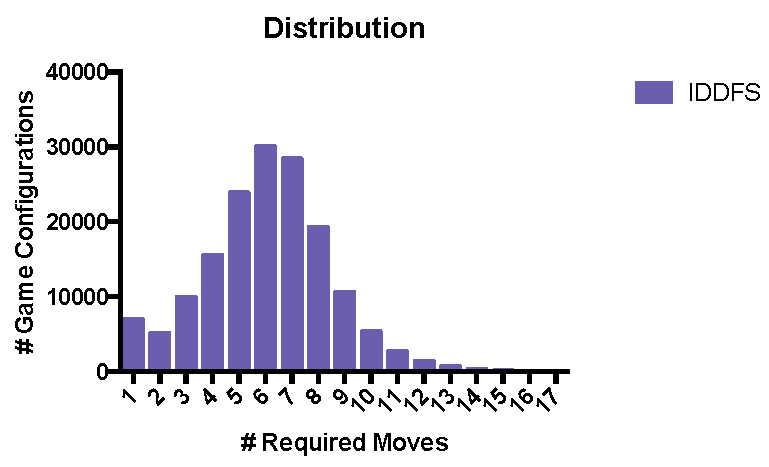
\includegraphics[width=0.7\linewidth]{img/dist.pdf}
\caption{The distribution of game configurations. }
\label{fig:dist}
\end{figure}

As shown in figure \ref{fig:hitrate}, the naive algorithm reaches the 40
seconds limit at about 13 moves while the IDDFS solves every
configuration. Also, the stateless and graph solutions follows each
other closely with a 5-10\% better hitrate for the latter. However, as
the game configurations become more complex, the hitrate drops to
\textasciitilde{}50\% for both solutions. Even though it seems that the
hitrate is low, the graph algorithms have a total accuracy close to 90\%
while the stateless algorithm solves the game in \textasciitilde{}80\%
of the game configurations as shown in figure \ref{fig:total_hitrate}.

\begin{figure}[htb]
\centering
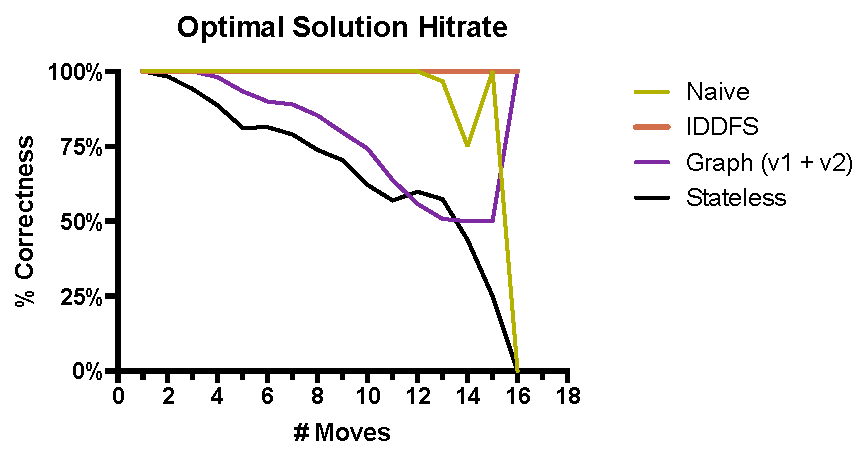
\includegraphics[height=0.25\textheight,width=0.7\textwidth,keepaspectratio]{img/hitrate.pdf}
\caption{The hitrate as a function of required number of moves.}
\label{fig:hitrate}
\end{figure}

\begin{figure}[htb]
\centering
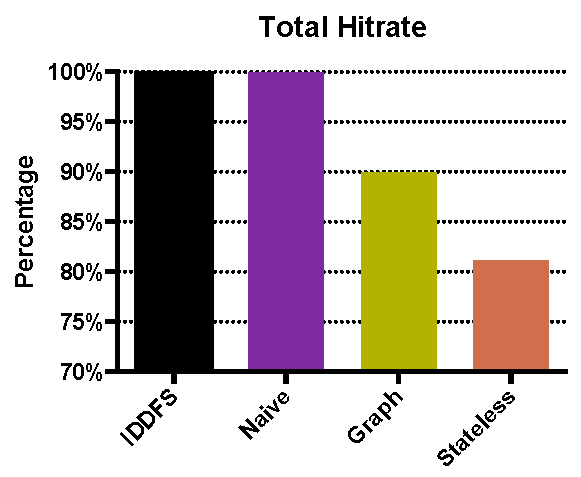
\includegraphics[height=0.25\textheight,width=0.7\textwidth,keepaspectratio]{img/total_hitrate.pdf}
\caption{The total hitrate as a percentage.}
\label{fig:total_hitrate}
\end{figure}

In figure \ref{fig:avg_optimal} the average running time is plotted as a
function of the required number of moves for the given game
configuration. The naive algorithm is the slowest algorithm by several
degrees and has been been left out. The stateless algorithm uses 1-2 ms
per solution indifferent to the number of required moves while the graph
v2 algorithm is considerable faster than the IDDFS at nine moves
required and higher.

\begin{figure}[htb]
\centering
\begin{minipage}{0.45\linewidth}
\centering
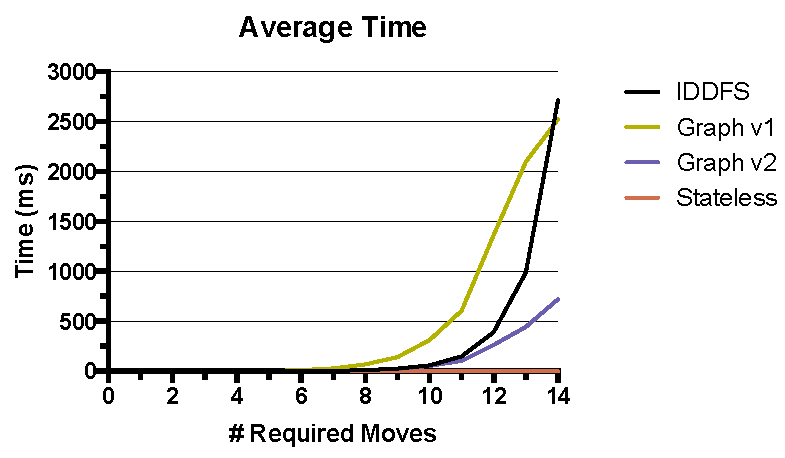
\includegraphics{img/avg_optimal.pdf}
\caption{The average running time as a function of required number of moves.}
\label{fig:avg_optimal}
\end{minipage}
\quad
\begin{minipage}{0.45\linewidth}
\centering
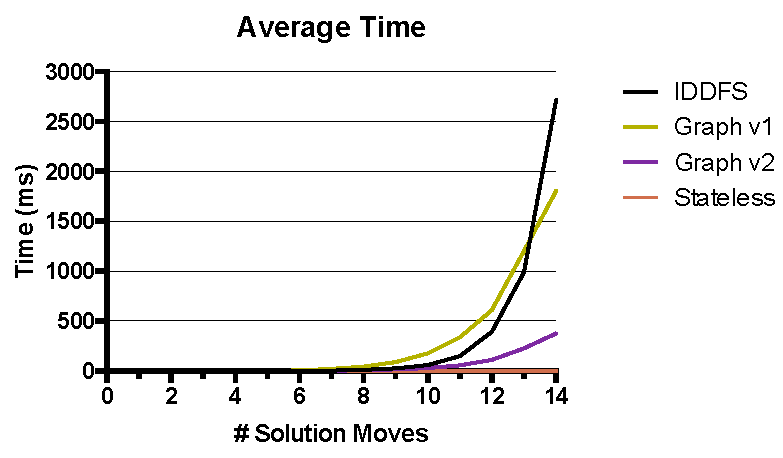
\includegraphics{img/avg_solution.pdf}
\caption{The average running time as a function of number of moves given by the result.}
\label{fig:avg_solution}
\end{minipage}
\end{figure}

Several results for the graph algorithms are not optimal and therefore
the average running time given in figure \ref{fig:avg_optimal} includes
results where the algorithms investigated more moves than actually
required. In figure \ref{fig:avg_solution} only the running time of
results where the graph algorithms found the optimal solutions are
compared. The stateless algorithm is omitted given the running time is
not affected by the required number of moves.

All data is available on appendix \ref{app:testdata}.

\subsection{Analysis}\label{analysis-3}

The running time of each algorithm corresponds well to the theoretical
analysis. All algorithms depending on the branching factor uses a
considerable amount of time as the complexity of the game configurations
increases. For the stateless algorithm, the worst case running time is
constant given the fixed size of the board, which also shows in the
results.

For the given game board, the result of 80\% of the game configurations
can be found in constant worst case running time.

It is clear that the optimizations applied to the graph algorithm have
affected the average running time consideredly. The extra cost of
precomputing the minimum moves is not a considerable factor. Comparing
the two graph algorithms, the increased performance of the graph v2 is
an exponential function of the number of moves. This corresponds well to
the actual optizmizations applied.

An interesting fact is that the graph v2 algorithm outperforms the IDDFS
on solutions with 9 or higher required number of moves. For solutions
where the graph v2 algorithm found the optimal solution, it outperforms
IDDFS on game configurations with 8 or higher required number of moves.
On solutions which required 16 moves, the graph v2 is faster with about
a factor 7.5 if considering only the cases where the graph v2 found the
optimal result.

However, the results also show that as the graph v2 and the stateless
algorithms outperform the IDDFS algorithm on solutions with nine or
higher required number of moves, the hitrate for each algorithm
decreases fast. Therefore, in the search space where the proposed
algorithms outperforms the known solutions, their reliability drops.

\section{Future Work}\label{future-work}

Given the results of my work, I would like to propose several
improvements and optimizations.

\subsection{Performance Tests}\label{performance-tests}

The performance tests are conducted on the same game board. However, it
would be interesting to investigate other game boards with a different
distribution of game configurations per required number of moves and how
it affects the running time of each proposed algorithm.

As the prototypes are implemented in Java, the algorithms could be
implemented in C/C++ for increased performance while several
machine-aware techniques could be used to optimize all algorithms in
general.

\subsection{Stateless}\label{stateless-1}

In few cases, the stateless algorithm returns a lower solution than
actually possible. This means that there exists cases that are not
accounted for, and these would have to be included in the assumptions.
If these cases can be included without affecting the running time, the
stateless algorithm will always guaranteee an upper limit for the
required number of moves. If this is the case, it can be included in
other algorithms and used to prune the search field.

\subsection{Graph}\label{graph}

During my tests I found that the BFS visits \textasciitilde{}60 nodes
for graph v1, while for graph v2 it only visits \textasciitilde{}15 on
average. This number directly depends on the number of reachable fields
on the board which again depends upon the number of obstacles. A more
precise worst case running time analysis could be proposed. This would
depend on a function of the number of fields and the number of obstacles
on the board instead of the number of nodes.

Another interesting improvement would be to move all robots including
the \emph{GR}. This would increase the branching factor, but the graph
algorithm would guarantee an optimal solution. Given the results of the
performance tests when comparing the average running time when the graph
algorithms found the optimal solution, there is still a considerable gap
between the IDDFS and the graph v2. A tradeoff between increasing the
running time while guaranteeing the optimal solution could be of
interest.

The pruning techniques introduced in the graph v2 could be improved.
They are not truely applied before the first time the BFS hits goal.
Thus, the graph v2 relies on finding an upper limit before the pruning
techniques works optimally. If the stateless algorithm can be improved
to guarantee an upper limit for the required number of moves, this might
be implemented into the graph algorithm when solving complex game
configurations, setting an upper bound for the search field and initiate
the pruning earlier.

\subsection{IDDFS}\label{iddfs}

The IDDFS could introduce the stateless algorithm on the more complex
game configurations to improve overall performance and skipping some
intermediate levels of deepening. However, given the incrementing nature
of the algorithm, it does not benefit the same way as the graph v2 does.
Depending on the inaccuracy of the stateless algorithm, this improvement
could improve the running time on the more complex algorithms.

\newpage

\appendix
\section{Game Board} \label{app:gameboard}

\begin{figure}[h]
\centering
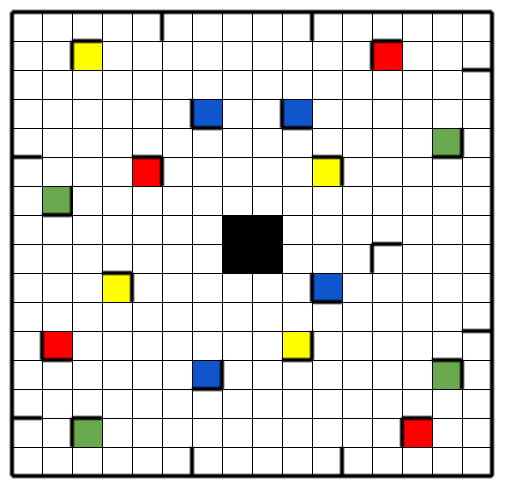
\includegraphics[height=1\textheight,width=1\textwidth,keepaspectratio]{img/gameboard.png}
\caption{The game board used for testing. The thick lines are obstacles. The colored fields are goals in the given color. The robots can be placed on all white fields.}
\label{fig:gameboard}
\end{figure}\newpage

\begin{landscape}
\section{Test Results} \label{app:testdata}

\begin{table}[h]
    \begin{tabular}{lllllllllllllllll}
        \toprule
        1 & 2 & 3 & 4 & 5 & 6 & 7 & 8 & 9 & 10 & 11 & 12 & 13 & 14 & 15 & 16 &      17 \\
        \midrule
        6958 & 5100 & 9920 & 15503 & 23860 & 30027 & 28370 & 19251 & 10579 &
        5309 & 2699 & 1380 & 688 & 264 & 78 & 13 & 1\\
        \bottomrule
    \end{tabular}
    \caption{The distribution of game configurations per required number of fields.}
\end{table}
\begin{table}[h]
    \begin{tabular}{llllllllllllllll}
        \toprule
        1 & 2 & 3 & 4 & 5 & 6 & 7 & 8 & 9 & 10 & 11 & 12 & 13 & 14 & 15 & 16\\
        \midrule
        6958 & 5100 & 9920 & 15503 & 23860 & 30027 & 28370 & 19251 & 10579 &
        5309 & 2699 & 1380 & 688 & 264 & 78 & 13\\
        \bottomrule
    \end{tabular}
    \caption{Average running times as a function of required moves. All numbers are in \emph{ms}.}
\end{table}
\end{landscape}\newpage

\begin{longtable}[c]{@{}lllllllllllllll@{}}
\caption{Average running times as a function of required moves where the
optimal solution was found. All numbers are in
\emph{ms}.--\textgreater{}}\tabularnewline
\toprule
Algorithm & 1 & 2 & 3 & 4 & 5 & 6 & 7 & 8 & 9 & 10 & 11 & 12 & 13 &
14\tabularnewline
\midrule
\endfirsthead
\toprule
Algorithm & 1 & 2 & 3 & 4 & 5 & 6 & 7 & 8 & 9 & 10 & 11 & 12 & 13 &
14\tabularnewline
\midrule
\endhead
IDDFS & 0 & 0 & 0 & 0 & 0 & 1 & 4 & 10 & 26 & 58 & 149 & 390 & 989 &
2714\tabularnewline
Graph v1 & 0 & 0 & 0 & 0 & 2 & 7 & 20 & 44 & 89 & 175 & 335 & 608 & 1200
& 1804\tabularnewline
Graph v2 & 0 & 0 & 0 & 0 & 0 & 1 & 3 & 7 & 15 & 28 & 57 & 112 & 227 &
375\tabularnewline
Stateless & 0 & 0 & 0 & 0 & 0 & 1 & 3 & 7 & 15 & 28 & 57 & 112 & 227 &
375\tabularnewline
\bottomrule
\end{longtable}

\end{document}
